\documentclass[english]{article}

\usepackage{arxiv}

\usepackage[utf8]{inputenc} % allow utf-8 input
\usepackage[T1]{fontenc}    % use 8-bit T1 fonts
\usepackage{hyperref}       % hyperlinks
\usepackage{url}            % simple URL typesetting
\usepackage{booktabs}       % professional-quality tables
\usepackage{amsfonts, amsmath}       % blackboard math symbols
\usepackage{nicefrac}       % compact symbols for 1/2, etc.
\usepackage{microtype}      % microtypography
\usepackage{cleveref}       % smart cross-referencing
\usepackage{lipsum}         % Can be removed after putting your text content
\usepackage{graphicx}
\usepackage{doi}
\usepackage{babel}
\usepackage{csquotes}


% Bibliography
\usepackage[%
  backend=biber,%
  backref=false,%
  giveninits=true,%
  autocite=inline,%
  sorting=none,% in order of occurence. Other option: nyt (name year title)
  sortcites=true,%
  mincitenames=1,%
  maxcitenames=2,%
  maxbibnames=10,%
  doi=false,%
  isbn=false,%
  url=false,%
  natbib=true,
]{biblatex}

\addbibresource{references.bib}

\title{Training Dense Object Nets While Not Training Dense Object Nets}

% Here you can change the date presented in the paper title
%\date{September 9, 1985}
% Or remove it
%\date{}

\author{ {Kanishk Navale, Ralf Gulde, Marc Tuscher} \\
	Sereact, \\
	Stuttgart, Germany \\
	\texttt{firstname.lastname@sereact.ai} \\
}

\begin{document}
\maketitle

\begin{abstract}
	We propose a framework to train Dense Object Nets (DON) with no intent to train DON;
	instead, we mine the dense visual object descriptors produced by DON while training another
	network unrelated to creating dense visual object descriptors. The dense visual object descriptors
	from the DON are object view-invariant, configuring and generalising the object's
	geometrical structure. However, an object image pair is required to train DON with the
	corresponding mapping, and recent research developments proves that the DON is as better as the number
	of correspondence supplied to it while training. The computation costs increase as the number
	of image-pair correspondences increases with the descriptor dimension, limiting one to produce
	descriptors of less dense dimension. Our framework does not require any image-pair correspondence mapping.
	It yields denser visual descriptors while consuming lesser computation resources while not compromising
	the robustness of the dense visual object descriptors compared to DON.

\end{abstract}

% keywords can be removed
\keywords{Dense Object Nets \and Second keyword \and More}


\section{Introduction}
As of this writing, the ideal object representation for robot grasping and manipulation tasks is yet unknown.
The existing representations may not be the best for tackling more complex tasks as they lack actual
object information belonging to the same class and configuration (shape, color and size).
In industrial robot-based automation, the objects are specifically coded for their visual features using 2D and 3D vision systems.
The downside of this lies in the fact that the robot has to be taught to pick every other part with its visual representation.
This process comes with the tedious schedule of teaching the robot to pick every part
irrespective of the part's configuration, and viewpoint. The solution lies in using artificial intelligence (AI) equipped robots.
A deep learning neural network (DNN) is based on artificial neurons capable to learning a task and is good as the task related
data it is trained on. The data used to train DNN is often expensive as it requires engineered features that DNN can predict or regress.
SIFT~\cite{sift}, SURF~\cite{bay2008speeded} and ORB~\cite{rublee2011orb} produce dense local descriptors of an object in an image
and serve as target features to train DNN
to yield object representation for robot grasping furthermore, these features computed by \parencites{sift}{bay2008speeded}{rublee2011orb} come with its own inert
limitations and cannot generalize objects well. Our interests of work is on reducing efforts to develop hand engineered features to train DNN
and developing DNN that can generalize plathora of objects such that we spend less time teaching robot how to tend objects in realtime.


In \citeyear{florence2018dense}, \citeauthor{florence2018dense}~\cite{florence2018dense} introduced a novel visual
object representation to the robotics community,  terming it ``dense visual object descriptors''. DON, an aritificial intelligence
framework proposed by
\Citeauthor{florence2018dense}~\cite{florence2018dense} produces dense visual object descriptors. In detail, the DON converts every pixel in the
image ($I[u, v] \in \mathbb{R}^3$) to a higher dimensional embedding ($I_D[u, v] \in \mathbb{R}^D$) such that $D \in \mathbb{N}^+$
which are nothing but dense local descriptors
of that pixel respective to the image. The dense visual object descriptor generalize an object up to a certain extent and have been recently
applied to rope manipulation \cite{rope-manipulation},
block manipulation \cite{block-manipulation}, robot control \cite{florence2019self}, fabric manipulation \cite{fabric-manipulation} and
robot grasp pose estimation \parencites{kupcsik2021supervised}{adrian2022efficient}. \citeauthor{suwajanakorn2018discovery}~\cite{suwajanakorn2018discovery}
propose self-supervised geometrically consistent keypoints, exploring the idea of optimizing a representation
based on a sparse collection of keypoints or landmarks, but without access to keypoint annotations. The authors of \cite{suwajanakorn2018discovery}
devise an end-to-end geometric reasoning framework
first introduced by \cite{levine2016end} to regresses a set of geometrically consistent keypoints coined as KeypointNet.
This means that KeypointNet is capable of generalizing objects without the need of hand engineered features.
\citeauthor{suwajanakorn2018discovery}~\cite{suwajanakorn2018discovery} show that using two unique objective loss
functions, namely, a relative pose
estimation loss and a multi-view consistency goal, uncovers the consistent keypoints across multiple views and object instances.
Their affine translation-equivariant design may extend to
previously unknown object instances trained on ShapeNet \cite{chang2015shapenet} dataset.

At first, we present modifications to the DNN inspired from \cite{florence2018dense} and \cite{suwajanakorn2018discovery} such that we seemlessly
train and mine object representations composed of object generalizing dense local descriptors while training for KeypointNet task. Second, we develop synthetic
dataset using \cite{blenderproc} to train the DNN and prove that
the mined dense local descriptors from our framework is as robust as dense visual object descriptors produced from DON while consuming less computation resources.
Additionally, we demonstrate an self-supervised framework to train DON with semantically equivalent objects which is not
previously demonstrated in \parencites{florence2018dense}{florence2020dense}{kupcsik2021supervised}{adrian2022efficient}{hadjivelichkov2021fully}{nerf-Supervision} to train DON.

\section{Related Work}
We are solely interested in computing dense visual object descriptors of an object.
The DON training strategy in \cite{florence2018dense} relies on the depth information for computing correspondences in an image pair using
camera intrinsics and pose information \cite{hartley2003multiple}.
However, when employing consumer-grade depth cameras for capturing the depth information,
the depth cameras capture noisy depth in cases of tiny, reflecting objects, which are common in
industrial environments. In the meantime, \citeauthor{kupcsik2021supervised}~\cite{kupcsik2021supervised} used Laplacian Eigenmaps \cite{belkin2003laplacian}
to embed a 3D object model into an optimally generated embedding space acting as an target to train DON in a supervised fashion.
The optimal embeddings brings in more domain knowledge by associating 3D object model to images views.
\citeauthor{kupcsik2021supervised}~\cite{kupcsik2021supervised} efficiently apply it to smaller, texture-less and
reflective objects by eliminating the need of the depth information. \citeauthor{kupcsik2021supervised}~\cite{kupcsik2021supervised}
further compare training strategies for producing 6D grasps for industrial objects and show that a unique supervised training approach
increases pick-and-place resilience in industry-relevant tasks.

\citeauthor{florence2020dense}~\cite{florence2020dense} has found that the pixelwise contrastive loss function used to train DON might not perform well if a computed
correspondence is spatially inconsistent (analogously to the case of noisy depth information). This further highlights that the precision
of contrastive-trained models can be sensitive to the
relative weighting between positive-negative sampled pixels. Instead, the \citeauthor{florence2020dense}~\cite{florence2020dense} introduces a new continuous
sampling-based loss function called ``Pixelwise Distribution Loss''.
The pixelwise distribution loss is much more effective as it is a smooth continuous pixel space sampling method compared to the
discrete pixel space sampling method based on pixelwise contrastive loss.
The pixelwise distribution loss regresses a set of probability distribution heatmaps aiming to minimize the divergence between the predicted
heatmap and the ground truth heatmap mitigating errors in correspondences. Futhermore, the pixelwise distribution loss does not
need non-matching correspondences compared to the
the pixelwise contrastive loss.
Differently, \citeauthor{hadjivelichkov2021fully}~\cite{hadjivelichkov2021fully} extends the DON training using semantic correspondences between objects in multi-object
or cluttered scenes overcoming the limitations of \parencites{hartley2003multiple}{belkin2003laplacian}.
The authors, \citeauthor{hadjivelichkov2021fully}~\cite{hadjivelichkov2021fully} employ offline unsupervised clustering based on confidence in object similarities to generate hard and soft correspondence labels.
The computed hard and soft labels lead DON in learning class-aware dense object descriptors, introducing hard and soft margin constraints in the proposed pixelwise contrastive loss to train DON.
Further eliminating the need for camera pose and intrinsic information along with depth information to compute correspondences in an image pair, \citeauthor{nerf-Supervision}~\cite{nerf-Supervision} used
NeRF~\cite{mildenhall2021nerf} to train DON. The NeRF~\cite{mildenhall2021nerf} recreates a 3D scene from a sequence of images captured by the smartphone camera. The correspondences are extracted from
the synthetically reconstructed scene to train DON.
Recently, based on SIMCLR inspired frameworks~\parencites{chen2020simple}{zbontar2021barlow},
\citeauthor{adrian2022efficient}~\cite{adrian2022efficient} introduced similar architecture and another novel loss function called
``Pixelwise NT-Xent loss'' to train DON more robustly.
The pixelwise ntxent loss consumes synthetic correspondences independent of depth cameras computed from image augmentations to train DON.
\citeauthor{adrian2022efficient}'s experiments show that the novel loss function is invariant with respect to the batch size.
Additionally adopted ``$PCK@k$''
metric has been adopted as in preceedings \parencites{chai2019multi}{fathy2018hierarchical} to evaluate and benchmark
DON on cluttered scenes previously not benchmarked.

In the proposed framework we do not use any loss functions in
\parencites{florence2018dense}{florence2020dense}{kupcsik2021supervised}{adrian2022efficient}{hadjivelichkov2021fully}{nerf-Supervision} to train DON
however we adopt the network architecture from \cite{florence2018dense} and train on the task of the ``KeypointNet''\cite{suwajanakorn2018discovery}
with adaption of the loss functions proposed in \parencites{suwajanakorn2018discovery}{zhao2020learning}.

\section{Methodology}
\subsection{DNN Framework and Mining Methodology}

As a backbone, we employ ResNet-34 architecture \cite{resnet}.
We preserve the last dense feature layer in the ResNet-34 DNN
and remove the last flatten feature in the forward method and linear layer that is popularly used for image classification tasks.
The backbone downsamples the RGB image $I_{RGB} \in \mathbb{R}^{H \times W \times 3}$
to dense features $I_d \in \mathbb{R}^{h \times w \times D}$
such that $ h \ll H, w \ll W \text{ and } D \in \mathbb{N}^+$.
We directly upsample the dense features from the identity layer as illustrated in the Figure~\ref{fig:modified_dnn} in page~\pageref{fig:modified_dnn} as follows:
\begin{equation}
    f_U: I \in \mathbb{R}^{h \times w \times D} \rightarrow I_D \in \mathbb{R}^{H \times W \times D},
\end{equation}
the upsampled dense features substitutes as dense visual local descriptors produced from the DON.
Similarly as in \cite{suwajanakorn2018discovery}, we stack spatial-probability regressing layer and
depth regressing layer on top of the identity layer to predict $N \in \mathbb{N}^+$ number of keypoint's spatial-probability as follows:
\begin{equation}
    f_S: I_d \in \mathbb{R}^{h \times w \times D} \rightarrow I_s^N \in \mathbb{R}^{h \times w \times N} \text{ , such that } \sum^{h} \sum^{w} I_s^N = 1.0^N,
\end{equation}
and depth as follows:
\begin{equation}
    f_D: I_d \in \mathbb{R}^{h \times w \times D} \rightarrow I_{\hat{d}} \in \mathbb{R}^{h \times w \times N}.
\end{equation}

We incorporate continuous sampling method $f_E$ from \parencites{florence2020dense}{suwajanakorn2018discovery}
to convert the upsampled predicted spatial-probability and depth of a keypoint to spatial-depth expectation as follows:
\begin{equation}
    f_E \circ g_E:[I_s, I_{\hat{d}}] \rightarrow [u, v, d]^T \in \mathbb{R}^3 \text{ , where }  g_E: I \in \mathbb{R}^{h \times w \times N} \rightarrow I \in \mathbb{R}^{H \times W \times N}.
\end{equation}
Furthermore, we train the DNN in a twin architecture fashion as depicted in the Figure~\ref{fig:twin_architecture}
in page~\pageref{fig:twin_architecture} as proposed in
\parencites{chen2020simple}{zbontar2021barlow}{florence2018dense}{florence2020dense}{kupcsik2021supervised}{adrian2022efficient}{hadjivelichkov2021fully}{nerf-Supervision}
on the KeypointNet task.

\begin{figure}[htb]
    \centering
    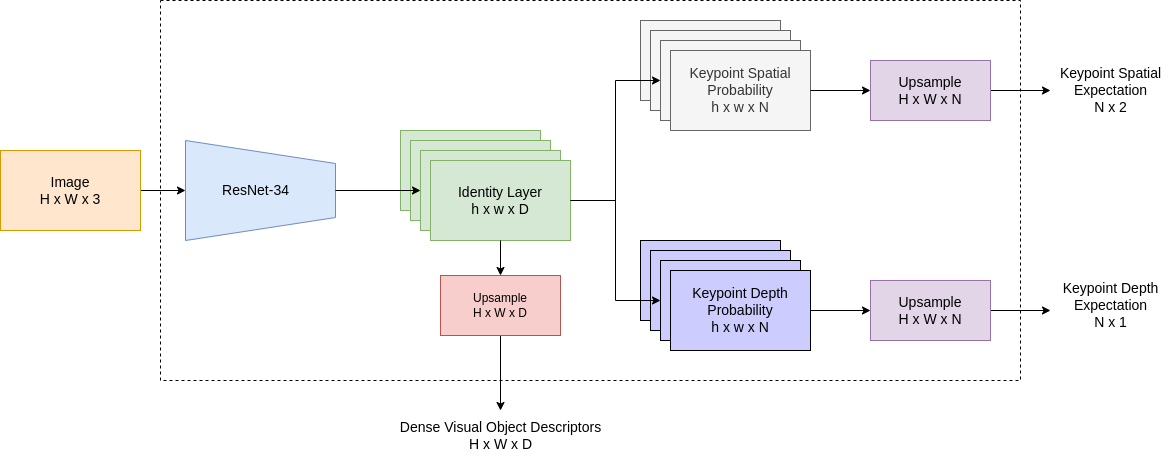
\includegraphics[scale=0.3]{images/arch.png}
    \caption{Illustration of novel DNN architecture designed to efficiently compute and seamlessly extract dense visual object descriptors.
        During inference we extract dense visual object descriptors directly from the network and ignore predicted spatial-depth expectation of the keypoints.}
    \label{fig:modified_dnn}
\end{figure}

\begin{figure}[htb]
    \centering
    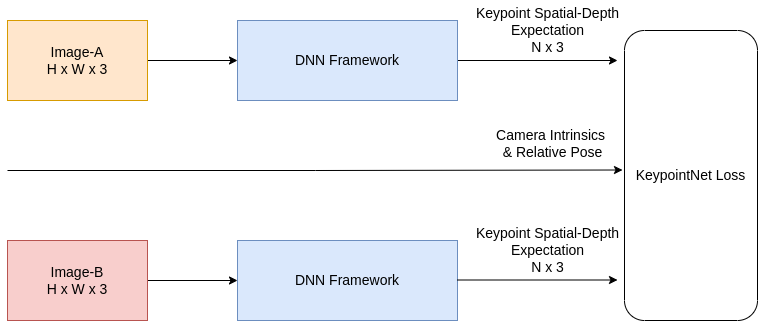
\includegraphics[scale=0.3]{images/twin.png}
    \caption{Depiction of twin DNN architecture's training strategy.}
    \label{fig:twin_architecture}
\end{figure}






\subsection{Loss Function Modifications}

For training, we directly adopt silhoutte consistency loss ($\mathcal{L}_{obj}$), variance loss ($\mathcal{L}_{var}$) and separation loss ($\mathcal{L}_{sep}$) functions from \cite{suwajanakorn2018discovery} to train the network on the keypoint prediction task.
However, we modify the multi-view consistent loss and relative pose estimation loss. In the case of multi-view consistency loss we
project the predicted spatial-depth expectation using camera intrinsics as follows:
\begin{equation}
    X_{cam} \in \mathbb{R}^{3 \times 1} = \mathcal{I}_{cam}^{-1}  \ [u, v, 1.0]^T \otimes d \text{ , where  } \ \mathcal{I}_{cam} \in \mathbb{R}^{3 \times 3} \text{ and }  u, v, d \in \mathbb{R}^+.
\end{equation}

Furthermore, we project the camera coordinates of the keypoints regressed on both images to the
world coordinates using camera transformation and compute Huber Loss~\cite{huber1992robust} represented as $\mathcal{H}$ in Equation~\ref{eqn:mvc} as multi-view consistency loss as follows:
\begin{equation}
    \label{eqn:mvc}
    \mathcal{L}_{mvc} \in \mathbb{R} = \mathcal{H}(\mathcal{T}_{C \rightarrow W}^A \hat{X}^A_{cam}, \mathcal{T}_{C \rightarrow W}^B \hat{X}^B_{cam}) \text{ , where  } \ \mathcal{T}_{C \rightarrow W} \in SE(3) \text{ and } \hat{X}_{cam}=[X_{cam}, 1.0]^T \in \mathbb{R}^{4 \times 1} ,
\end{equation}

this modification is geometrically more intuitive as all the keypoints projected from different camera viewpoints into world coordinates occupy the same value
addtionally, using Huber Loss creates smoother gradients to optimize the DNN compared to the original implementation of Euclidean distance.
In Equation~\ref{eqn:mvc} $SE(3) \in \mathbb{R}^{4 \times 4}$ is a ``Special Euclidean Group''~\cite{thurston2014three}.
We do not discard the relative transformation information to calculate the realative pose loss as suggested in \cite{suwajanakorn2018discovery}
and being influenced from \cite{zhao2020learning} we modified the relative pose loss as follows:
\begin{equation}
    \mathcal{L}_{pose} = \Vert log(\mathcal{T}_{truth}^{\dagger} \mathcal{T}_{pred}) \Vert \text{ , where  } \ log: SE(3) \rightarrow \mathfrak{se}(3) \text{ and } \mathcal{T}^{\dagger} = \begin{bmatrix}
        R^T & -R^T t \\
        0^T & 1
    \end{bmatrix} \in SE(3).
\end{equation}


\subsection{Controlled Dataset Engineering}

We have chosen the cap object for creating synthetic dataset as the cap mesh models are readily available in the ``Shapenet'' library~\cite{chang2015shapenet}
as it possess rich object information including textures.
Blenderproc~\cite{blenderproc} is used to generate the synthetic cap dataset by using of the 10 number of cap models from \cite{chang2015shapenet} library.
Futhermore, the caps are chosen such that each of them have distinct shapes, designs and colors.
For this controlled dataset, 100 random cameras are added in the environment with random poses capturing depth,
camera extrinsics information (referring to $\mathcal{T}_{C \rightarrow W}$ in Equation~\ref{eqn:mvc}) and object mask for each viewpoint for each cap model.
To make the training more robust such that networks are more object-centric, the images are additionally augmented with random backgrounds and noisy backgrounds
as depicted in Figure~\ref{fig:back_augmentations} in page~\pageref{fig:back_augmentations}
in addition to the color jitter and greyscale augmentations. For color jitter and greyscale augmentation we use available ``Torchvision''~\cite{marcel2010torchvision} library.


\begin{figure}[htb]
    \centering
    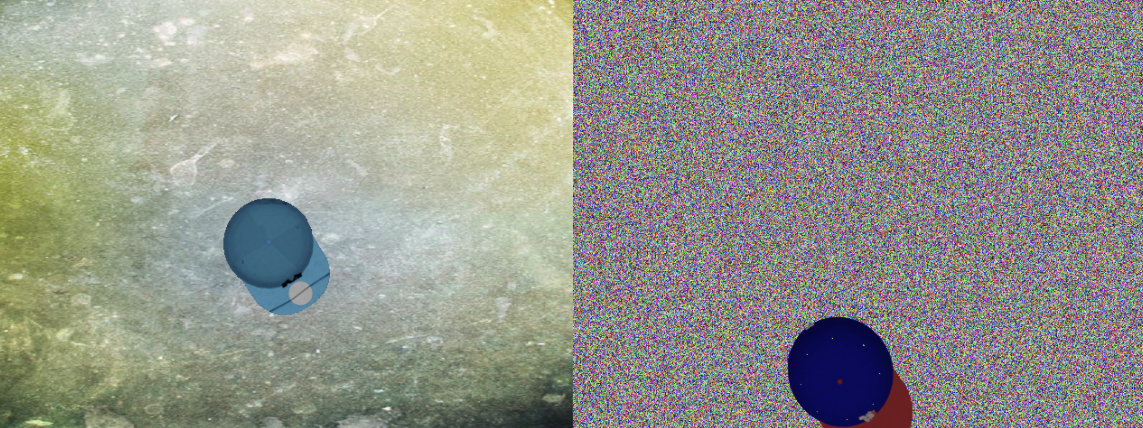
\includegraphics[scale=0.2]{images/back_augs.png}
    \caption{The image in the right illustrates the noisy background augmentation and the image in left depicts random background augmentation.}
    \label{fig:back_augmentations}

\end{figure}

\section{Results and Benchmarking}
We implemented out training and benchmarking using ``PyTorch-Lightning''\cite{falcon2019pytorch} and ``PyTorch''\cite{paszke2019pytorch} libraries.
Futhermore, we employ
``ADAM''\cite{kingma2014adam} optimizer to optimize our model for 1000 epochs with learning rate of
$\alpha = 10^{-3}, \beta_1 = 0.9 \text{ and } \beta_2 = 0.999$ with weight decay $\eta =10^{-6}$.
Addtionally, we reduce the learning rate by a factor of $0.9$ every 2500 opimtization steps.
We set the all the loss weights to 1.0 except variance loss weight to $w_{var} = 10^{-4}$ and mean reduce our batch-wise losses.
The proposed novel DNN model is benchamarked against standard DON model for computed dense visual object descriptors and
computation resources used where batch size plays a major influence.
For training standard DON model, we import training settings, evaluation
metrics and the method of generating synthetic correspondences as in
\cite{adrian2022efficient}\footnote{GitHub link to our implementation of generating synthetic correspondences: \url{https://github.com/KanishkNavale/Mapping-Synthetic-Correspondences-in-an-Image-Pair}}.


\printbibliography


\end{document}
